\documentclass[20pt,margin=1in,innermargin=-4.5in,blockverticalspace=-0.25in]{tikzposter}
\geometry{paperwidth=42in,paperheight=32.5in}
\usepackage[utf8]{inputenc}
\usepackage{amsmath}
\usepackage{amsfonts}
\usepackage{amsthm}
\usepackage{amssymb}
\usepackage{mathrsfs}
\usepackage{graphicx}
\usepackage{adjustbox}
\usepackage{enumitem}
\usepackage{color}
\usepackage[backend=biber,style=numeric]{biblatex}
\usepackage{uomtheme}
%%%%%%%%%%%%%%%
%\usepackage{nomencl}
%\makenomenclature
%%%%%%%%%%%%%%%%%
%\usepackage[colorlinks]{hyperref}
%\usepackage[symbols,nogroupskip,sort=none]{glossaries-extra}
%\glsxtrnewsymbol[description={position}]{x}{\ensuremath{x}}
%\glsxtrnewsymbol[description={velocity}]{v}{\ensuremath{v}}
%\glsxtrnewsymbol[description={acceleration}]{a}{\ensuremath{a}}
%\glsxtrnewsymbol[description={time}]{t}{\ensuremath{t}}
%\glsxtrnewsymbol[description={force}]{F}{\ensuremath{F}}
%%%%%%%%%%%%%
\newcommand{\bslash}{\char`\\}

\usepackage{mwe} % for placeholder images

\addbibresource{refs.bib}

% set theme parameters
\tikzposterlatexaffectionproofoff
\usetheme{UoMTheme}
\usecolorstyle{UoMStyle}

\usepackage[scaled]{helvet}
\renewcommand\familydefault{\sfdefault} 
\usepackage[T1]{fontenc}


\title{Surrogate model constructed using neural networks for the forward and inverse problems}
\author{Wenjuan (Tina) Zhang}
\institute{University of Colorado Denver}
\titlegraphic{
\includegraphics[width=0.04\textwidth]{QR.png}}

% begin document
\begin{document}
\maketitle
\centering
\begin{columns}
\column{0.32}
\block{Surrogate Model}{ 
\textbf{Problem:}\\
How to quantify the uncertainties when the mapping between the input and output spaces is not achievable, but can be approximated?\\

\noindent \textbf{Goal:}\\
Analyzes the convergence of probability densities solving uncertainty quantification problems using surrogate model.
}

\block{Example}{
Consider the following ODE:
\begin{align*}
y' &=-\lambda xy\\
y(0) &=1
\end{align*}
where $0.3\leq x\leq 0.7$, $\lambda$ is an uncertainty parameter.\\

\noindent \textbf{Exact Solution:}\\
 $$
 y(x,\lambda)=e^{-\lambda x^2/2}
 $$
}

\block{Forward UQ Problem}{
 Assume $\lambda\sim Beta(2,2)$,\\
 QoI is $Q(\lambda) = y(0.5;\lambda)$. \\
 
 \noindent \textit{For demonstration purpose, assume we do not know the exact solution describing the relation from $x$, $\lambda$ to $y$.}\\
 
%\noindent \textbf{Goal:}\\
%Analyze the convergence of push-forward densities solving the forward UQ problem using a sequence of approximate maps.\\

\noindent \textbf{Surrogate Model:}\\
Neural Network: 400 training data for $x$ is from $U[0.3,0.7]$; 400 training data for $\lambda$ is from $Beta(2,2)$.\\
The neural network is trained under different numbers of epochs, 1000, 2000, 5000, 10000, to create surrogate models \cite{1}.\\
%In \cite{cite:5}, the main result was the description of canonically $z$-invariant 


\textbf{\textcolor{blue}{Convergence of $L_2$ distance}}
\begin{tikzfigure}[L2 difference by using surrogate model.]
	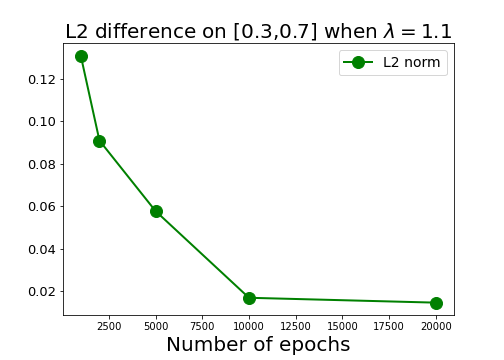
\includegraphics[width=0.5\linewidth]{1.png}
\end{tikzfigure}

\vspace{0.5cm}
\noindent \textit{Since our quantity of interest is uncertain due to the randomness from $\lambda$, to verify the convergence of push-forward densities using approximate maps, we create the error plot by using the $L^2$ distance on $[0.3,0.7]$ for a fixed $\lambda$ value 1.1.}\\

%\noindent \textbf{Conclusion:}\\
%The surrogate model constructed above converges as more epochs are being used.
%%Surrogate model converges in the $L^2$ sense.
%
}

\column{0.36}
\block{Forward UQ Problem (Continued)}{
\textbf{\textcolor{blue}{Convergence of push-forward density}}
\vspace{-1.5cm}
\begin{tikzfigure}[Push-forward density.]
	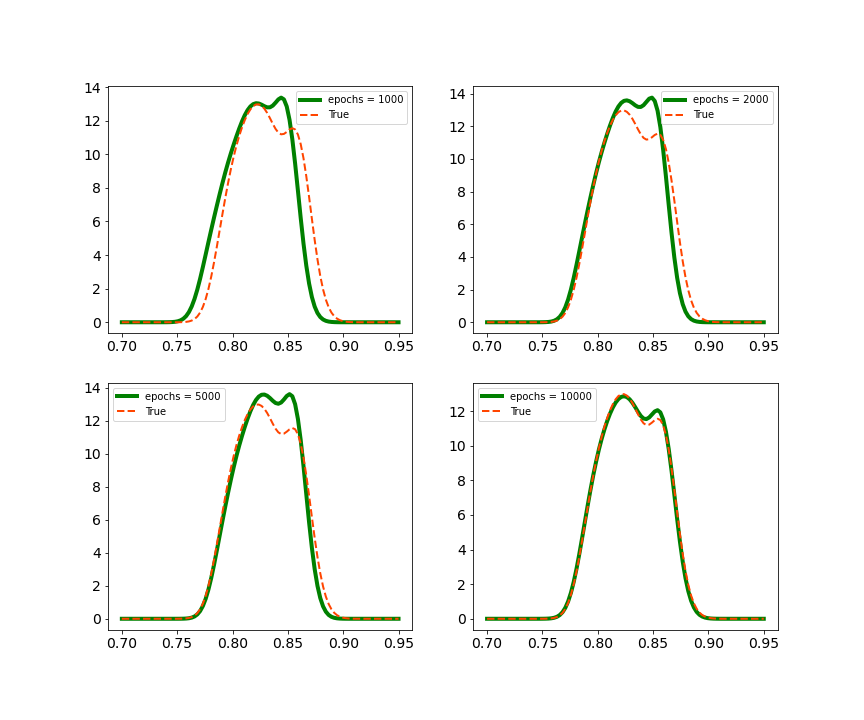
\includegraphics[width=0.7\linewidth]{2.png}
\end{tikzfigure}

\noindent \textbf{Conclusion:} \\
Surrogate model constructed using neural networks helps approximate true push-forward density.
}

\block{Intro to Data Consistent Inversion}{
\textbf{Data Consistent Inversion} is a novel framework that uses push-forward and pullback measures to ensure solutons are consistent with the observed distribution of data. \\

\begin{center}
\textbf{Data Consistent Inversion Approach}
\end{center}
\textbf{Using the exact model} \cite{2}:
$$
\pi_{\Lambda}^{\text{up}}(\lambda) = \pi_{\Lambda}^{\text{init}}(\lambda)\  \frac{\pi_{\mathcal{D}}(Q(\lambda))}{\pi_{\mathcal{D}}^{Q}(Q(\lambda))}
$$
\textbf{Using the surrogate model} \cite{3}:
$$
\pi_{\Lambda}^{\text{up},n}(\lambda) = \pi_{\Lambda}^{\text{init}}(\lambda)\  \frac{\pi_{\mathcal{D}}(Q_n(\lambda))}{\pi_{\mathcal{D}}^{Q_n}(Q_n(\lambda))}
$$

\textcolor{blue}{\textbf{Demonstration}}
\vspace{-1cm}
\begin{tikzfigure}[Data Consistent Inversion Method.]
	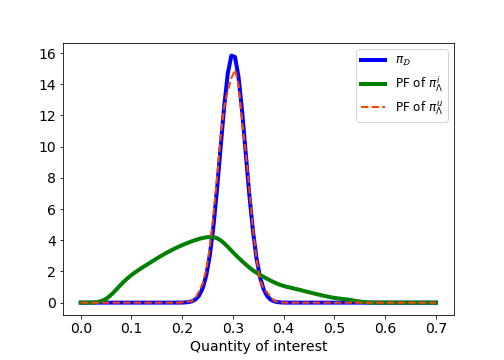
\includegraphics[width=0.56\linewidth]{3.png}
\end{tikzfigure}
}

\column{0.32}
\block{Inverse UQ Problem}{
\textbf{\textcolor{blue}{Convergence of updated density}}
%\vspace{-1.5cm}
\begin{tikzfigure}[L2 difference between true update and approximate update.]
	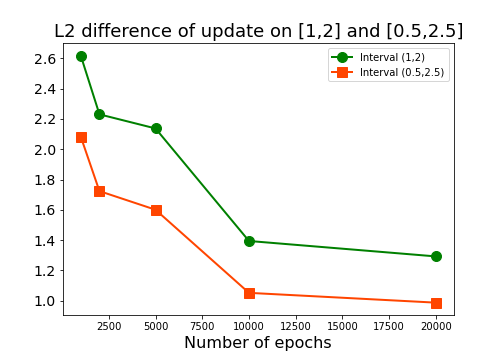
\includegraphics[width=0.5\linewidth]{4.png}
\end{tikzfigure}

\textbf{Conclusion:}\\
Surrogate model constructed using neural networks helps approximate true updated density.
}

\block{Notation}{
	\setlength{\tabcolsep}{12pt}
\renewcommand*{\arraystretch}{1.2}
\begin{center}
\begin{tabular}{lcl}
	\hline
	Notation & Description \\
	\hline
	$\lambda\in\Lambda$ & Parameter Space \\
	$\mathcal{D}$ & Observable Space \\
	$Q$ & Exact model \\
	$Q_n$ &$n$-th surrogate model \\
	$\pi_{\Lambda}^{\text{init}}$ & Initial density guess of $\lambda$\\
	$\pi_{\Lambda}^{\text{up}}$ & Update pullback density\\
	$\pi_{\Lambda}^{\text{up},n}$ & Approximate update pullback density using $Q_n$\\
	$\pi_{\mathcal{D}}$ &Observed density \\
	$\pi_{\mathcal{D}}^{Q}$ & Push-forward density\\
	$\pi_{\mathcal{D}}^{Q_n}$ & Approximate push-forward density\\
%	{\bf Big O(micron)}&$\mathcal{O}$ or $O$ \\
%	{\bf Big Omega}&$\Omega$ \\
%	{\bf Big Theta}&$\Theta$ \\
%	{\bf Small O(micron)}&$o$ \\
%	{\bf Small Omega}&$\omega$ \\
%	{\bf On the order of}&$\sim$ \\
	\hline
\end{tabular}
\end{center}
%	\printunsrtglossary[type=symbols,style=long]
%\nomenclature{$\lambda\in\Lambda$}{Parameter Space}
%\nomenclature{$\mathcal{D}$}{Observable Space}
%\nomenclature{$Q_n$}{$n$-th surrogate model}
%\nomenclature{$\pi_{\Lambda}^{u,n}$}{Update pullback density using $Q_n$}
%\nomenclature{$\pi_{\mathcal{D}}$}{Observed density}
%\nomenclature{$\pi_{\mathcal{D}}^{Q_n}$}{Push-forward density}
%\printnomenclature
}

%    \block{Acknowledgements}{
%        Lorem ipsum dolor sit amet, probo dolorem cu vis. Cu mei audire fabulas scriptorem, cu has clita fabulas. Sea id veritus maiorum indoctum, mea cu assum cetero. Ei posse movet maluisset vim.
%    }

\block{References}{
\vspace{-1em}
\begin{thebibliography}{}
	\bibitem{1}
	Lagaris, I., Likas, A., and Fotiadis, D.,
	\textit{Artificial Neural Networks for Solving Ordinary and Partial Differential Equations},
	\textit{IEEE Transactions on Neural Networks}, 9(5):987-1000, 1998.
	
	\bibitem{2} 
	Butler, T., Jakeman, J., and Wildey, T., 
	\textit{Combining push-forward measures and bayes’ rule to construct consistent solutions to stochastic inverse problems}, \textit{SIAM Journal on Scientific Computing}, 40(2):A984-A1011, 2018.
	
	\bibitem{3} 
	Butler, T., Jakeman, J., and Wildey, T., 
	\textit{Convergence of probability densities using approximate models for forward and inverse problems in uncertainty quantification},
	\textit{SIAM Journal on Scientific Computing}, 40(5):A3523–A3548, 2018.
	


\end{thebibliography}
%\bibliographystyle{siam}
%\bibliography{refs}
%\begin{footnotesize}
%\printbibliography[heading=none]
%\end{footnotesize}
}
\end{columns}
\end{document}